\section{Sample-Based Computation}
\label{sec:sampling}

%Stochastic PCA methods that iterate over small data samples either $i)$ execute for a pre-specified number of iterations or $ii)$ execute until convergence to the solution provided by classical PCA.
%To our knowledge, these existing termination conditions are not suitable when considering users' willingness to trade quality for downstream workload runtime.
%However, using these methods as a starting point,
We \red{augment our case study to} show that running PCA on data samples does not sacrifice DR quality, but that the number of samples required varies per dataset.
We then show how progressively increasing the sampling rate can help dynamically identify how much to sample a given dataset.

\subsection{Feasibility of Sampling}
Many real-world \red{datasets} are intrinsically low-dimensional, as evidenced by their rapid falloff in their eigenvalue spectrum.
A data sample thus captures much of the dataset's ``interesting'' behavior, so fitting a model over such a sample will generalize well. We verify this phenomenon by varying the target $TLB$ and examining the minimum number of samples required to obtain a $TLB$-preserving transform with output dimension $k$ equal to input dimension $\dvar$.

On average, across the considered UCR time series datasets, a sample of under $0.64\% (\text{up to } 5.5\%)$ of the input is sufficient for a $TLB$ of $0.75$, and under $4.15\% (\text{up to } 38.6\%)$ is sufficient for a $TLB$ of $0.99$.  
When this proportion is known a priori, we obtain up to \red{$91\times$ speedup} compared to a na\"ive implementation of PCA via SVD---with no algorithmic improvement. 


\subsection{Incremental, Progressive Sampling}
Sampling benefit is dataset-dependent; we must identify how large a sample suffices to compute high-quality transforms.
Figure~\ref{fig:progressive} shows how the dimensionality required to attain a given $TLB$ changes when we vary dataset and proportion of data sampled.
Increasing the number of samples provides lower dimensional transformations for the same quality.
However, this decrease in dimension plateaus as the number of samples increases.
Thus, we must determine when the downstream value of decreased dimension is overpowered by the cost of additional DR---that is, whether to sample to convergence (evaluated in Section~\ref{subsec:lesion}) or terminate early (e.g., at $0.3$ proportion of data sampled for SmallKitchenAppliances). 


\begin{figure}
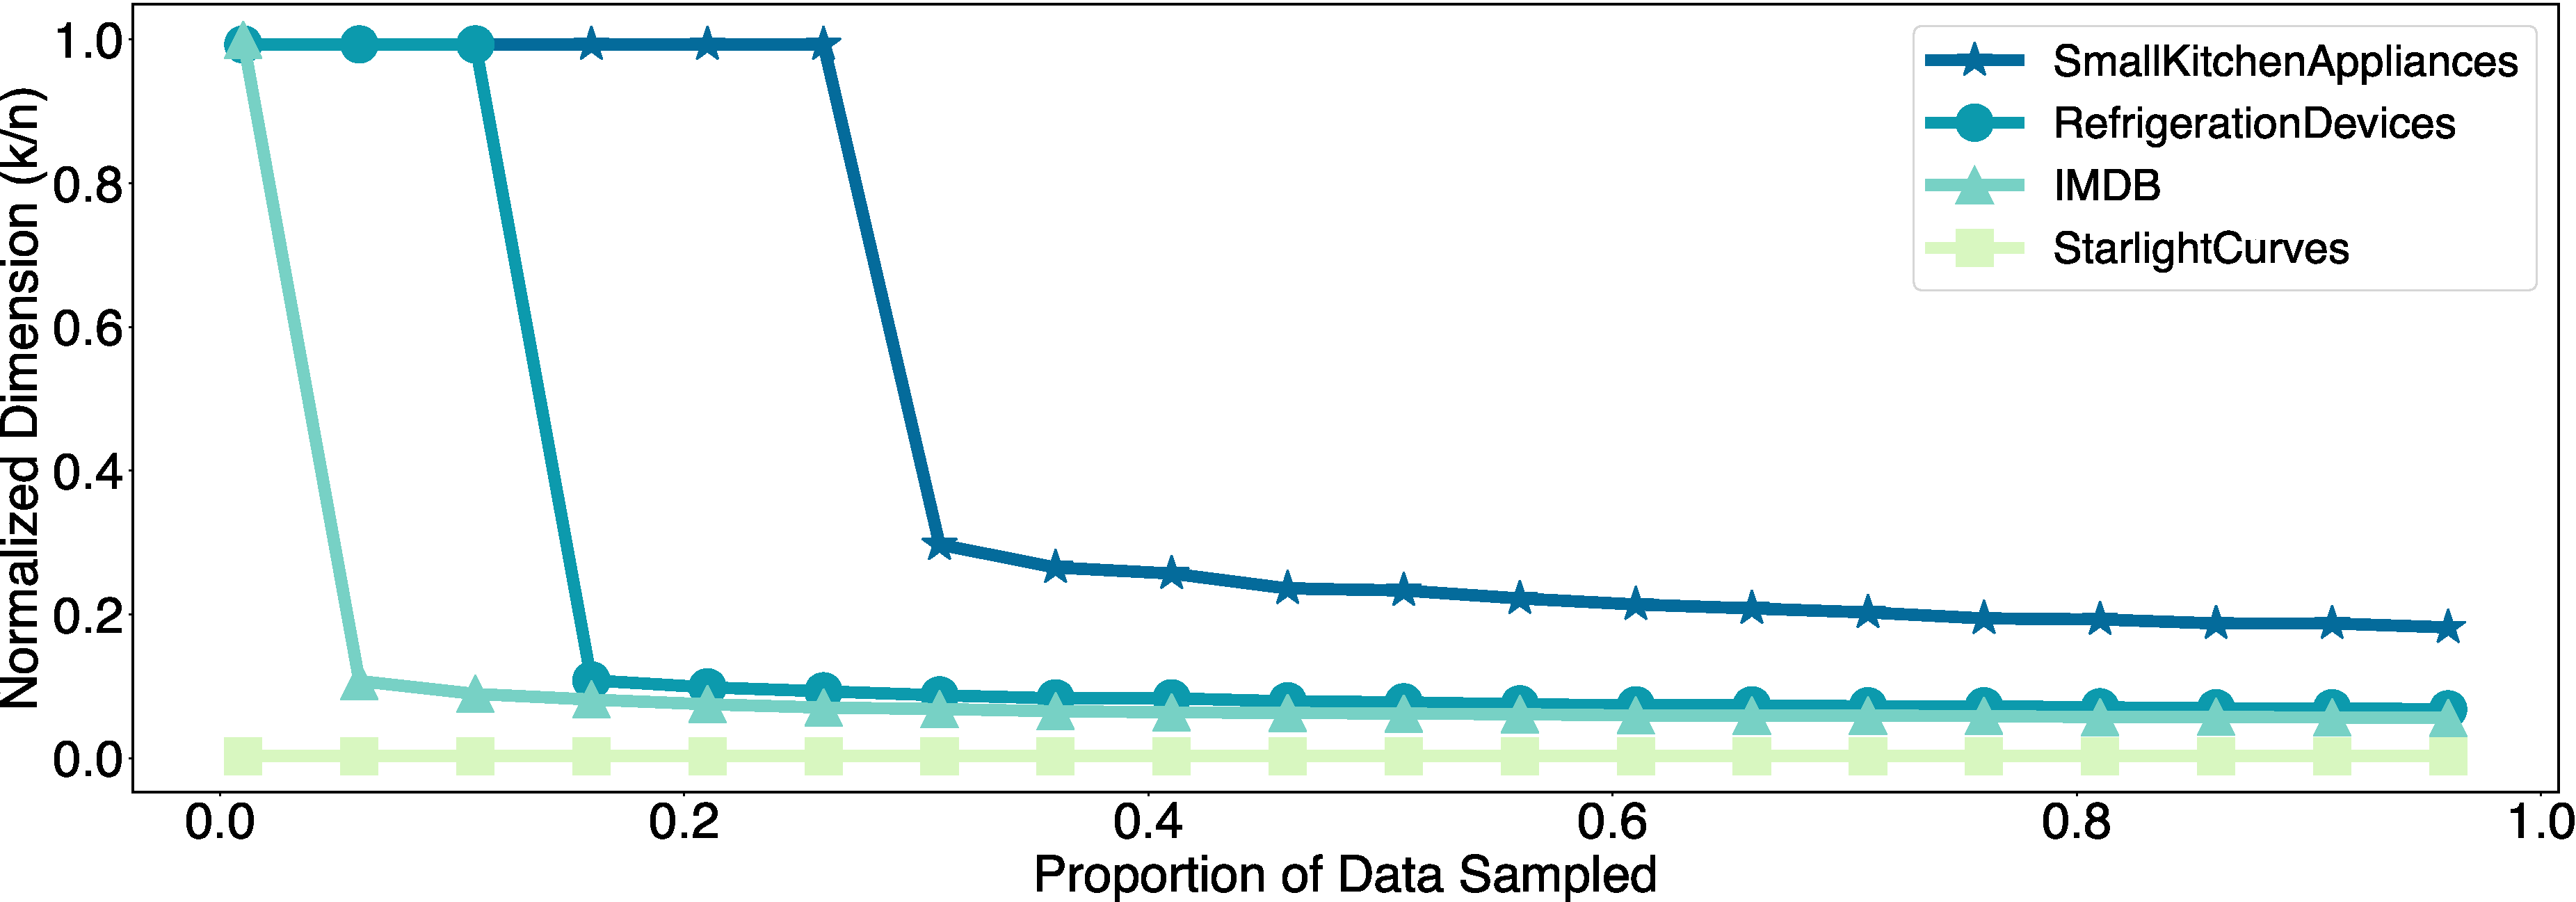
\includegraphics[width=\linewidth]{figs/progressive.pdf}
\caption[]{ Improvement in representation size for  $TLB = 0.80$ across three datasets. Higher sampling rates improve quality until reaching a state equivalent to running PCA over the full dataset ("convergence")}
\label{fig:progressive}
\end{figure}




